%%
%% Copyright 2022 OXFORD UNIVERSITY PRESS
%%
%% This file is part of the 'oup-authoring-template Bundle'.
%% ---------------------------------------------
%%
%% It may be distributed under the conditions of the LaTeX Project Public
%% License, either version 1.2 of this license or (at your option) any
%% later version.  The latest version of this license is in
%%    http://www.latex-project.org/lppl.txt
%% and version 1.2 or later is part of all distributions of LaTeX
%% version 1999/12/01 or later.
%%
%% The list of all files belonging to the 'oup-authoring-template Bundle' is
%% given in the file `manifest.txt'.
%%
%% Template article for OXFORD UNIVERSITY PRESS's document class `oup-authoring-template'
%% with bibliographic references
%%

%%%CONTEMPORARY%%%
\documentclass[unnumsec,webpdf,contemporary,large]{oup-authoring-template}%
%\documentclass[unnumsec,webpdf,contemporary,large,namedate]{oup-authoring-template}% uncomment this line for author year citations and comment the above
%\documentclass[unnumsec,webpdf,contemporary,medium]{oup-authoring-template}
%\documentclass[unnumsec,webpdf,contemporary,small]{oup-authoring-template}

%%%MODERN%%%
%\documentclass[unnumsec,webpdf,modern,large]{oup-authoring-template}
%\documentclass[unnumsec,webpdf,modern,large,namedate]{oup-authoring-template}% uncomment this line for author year citations and comment the above
%\documentclass[unnumsec,webpdf,modern,medium]{oup-authoring-template}
%\documentclass[unnumsec,webpdf,modern,small]{oup-authoring-template}

%%%TRADITIONAL%%%
%\documentclass[unnumsec,webpdf,traditional,large]{oup-authoring-template}
%\documentclass[unnumsec,webpdf,traditional,large,namedate]{oup-authoring-template}% uncomment this line for author year citations and comment the above
%\documentclass[unnumsec,namedate,webpdf,traditional,medium]{oup-authoring-template}
%\documentclass[namedate,webpdf,traditional,small]{oup-authoring-template}

%\onecolumn % for one column layouts

%\usepackage{showframe}

% line numbers
%\usepackage[mathlines, switch]{lineno}
%\usepackage[right]{lineno}

%%\theoremstyle{thmstyleone}%
%%\newtheorem{theorem}{Theorem}%  meant for continuous numbers
%%\newtheorem{theorem}{Theorem}[section]% meant for sectionwise numbers
%% optional argument [theorem] produces theorem numbering sequence instead of independent numbers for Proposition
%%\newtheorem{proposition}[theorem]{Proposition}%
%%\newtheorem{proposition}{Proposition}% to get separate numbers for theorem and proposition etc.
%%\theoremstyle{thmstyletwo}%
%%\newtheorem{example}{Example}%
%%\newtheorem{remark}{Remark}%
%%\theoremstyle{thmstylethree}%
%%\newtheorem{definition}{Definition}
\usepackage{url}
\usepackage{hyperref}
\usepackage[utf8]{inputenc}
\usepackage[T1]{fontenc}
\usepackage{tabularx}

\begin{document}


\pubyear{2025}
\appnotes{Report}

\firstpage{1}

\graphicspath{{Fig/}}

%\subtitle{Subject Section}

\title[Fine-Tuning LLM for Clinical Decision Support]{medLLM: Fine-Tuning a Medical language Model for Clinical Decision Support}

\author{Gaurika Chopra}
\author{Noah Garkisch}
\author{Neil Hinrichs}
\author{Willi Löther}
\author{Dominik Martens}
\author{Tejaswi Venkatesh}

\address[1]{\orgdiv{Department}, \orgname{Organization}, \orgaddress{\street{Street}, \postcode{Postcode}, \state{State}, \country{Country}}}
\address[2]{\orgdiv{Department}, \orgname{Organization}, \orgaddress{\street{Street}, \postcode{Postcode}, \state{State}, \country{Country}}}
\address[3]{\orgdiv{Department}, \orgname{Organization}, \orgaddress{\street{Street}, \postcode{Postcode}, \state{State}, \country{Country}}}
\address[4]{\orgdiv{Department}, \orgname{Organization}, \orgaddress{\street{Street}, \postcode{Postcode}, \state{State}, \country{Country}}}

\corresp[$\ast$]{Corresponding author. \href{email:email-id.com}{email-id.com}}

\received{Date}{0}{Year}
\revised{Date}{0}{Year}
\accepted{Date}{0}{Year}

%\editor{Associate Editor: Name}

%\abstract{
%\textbf{Motivation:} .\\
%\textbf{Results:} .\\
%\textbf{Availability:} .\\
%\textbf{Contact:} \href{name@email.com}{name@email.com}\\
%\textbf{Supplementary information:} Supplementary data are available at \textit{Journal Name}
%online.}

test


% \boxedtext{
% \begin{itemize}
% \item Key boxed text here.
% \item Key boxed text here.
% \item Key boxed text here.
% \end{itemize}}

\maketitle


\section{Introduction}
In the rapidly evolving field of medicine, doctors are required to process vast amounts of information to make well-informed decisions. However, accessing relevant medical literature can be time-consuming and challenging. This project aims to address this issue by developing a large language model designed to assist doctors in gathering crucial patient-related information efficiently.
The proposed model allows doctors to input a patient description as a prompt, after which it retrieves and summarizes relevant medical research papers. This process provides physicians with critical insights derived from medical literature. This approach enhances work efficiency, reduces cognitive load, and ensures that important information is readily accessible when needed.
To achieve this, our system employs a two-stage approach: retrieval and summarization. For the retrieval phase, we utilize RoBERTa, a robust Transformer-based model, to process the input prompt and identify the most relevant medical research articles from the PMC-Patients database. 
Once the relevant articles are retrieved, the summarization phase is handled using either Llama 3.2 1b instruct or Llama 3.3. We experimented with both models separately to determine which one provided the most accurate and useful summaries for clinical decision-making. Through comparative analysis, we assessed which model performed better in summarizing medical literature effectively for our use case.
This report outlines the development, training, and evaluation of the model, detailing its capabilities and limitations. Specifically, we discuss the dataset utilized for training, the preprocessing techniques employed, the symptom extraction process, the machine learning architecture, and the evaluation methods used to assess summarization quality. Furthermore, we examine the model’s performance and highlight areas for improvement.


\section{Methods}
\subsection{Dataset}
The PMC-Patients dataset is a large-scale dataset designed to support retrieval-based clinical decision support tasks [PMC dataset]. It is aggregated from PubMed Central articles, along with citation relationships. The key components of the dataset include patient summaries, which are text-based descriptions of patient cases sourced from PMC articles, a total of 3.1 million Patient-to-Article Relevance Annotations, connecting patient cases to relevant PubMed articles and 293,000 patient-to-patient similarity annotations which are identifying similar patient cases based on clinical characteristics. The PMC dataset is obtained by performing data cleaning; eliminating non-human cases, less than 10 word patient summaries and removal of columns with missing values. The dataset supports two primary retrieval based tasks in clinical decision support which are Patient-to-Article Retrieval, retrieving relevant scientific literature for a given patient summary as well as Patient-To-Patient Retrieval, that outputs similar patients from the dataset. 
With its structured annotations, PMC-Patients stands out as one of the largest publicly available datasets for patient-level information retrieval and clinical decision support.
The use of the PMC-Patients is beneficial in several ways. One argument is that with over 167,000 patient case summaries, that dataset covers a wide range of clinical scenarios, making it well-suited for training machine learning models. Beyond this, the high-quality relevance and similarity annotations enhance retrieval tasks. Additionally, the PMC-Patients dataset as an openly available dataset ensures transparency and reproducibility in research. The dataset also aligns with the aim to classify patients based on their descriptions to articles and retrieve the articles afterward.

As part of the data preparation process, the original PMC Patients dataset was first reduced to a manageable sample of 10,000 cases, prioritizing articles with open access. Patient information is organized using a unique patient ID, with a specific article assigned to each record via the associated PubMed ID (PMID). The Europe PMC Restful web services are used to check whether each article complies with Open Access standards [https://europepmc.org/RestfulWebService]. In this way, only those articles that are freely accessible are included in the further processing procedure. The data is then enriched with bibliographic information. For example, the title, DOI, authors, year of publication, journal and abstract are extracted in order to comprehensively map the context of the articles. For articles classified as open access, the URL of the complete PDF document is also determined, which enables direct access to the full text PDF file. In the next phase, the PDF documents of the selected articles are automatically downloaded and processed. The contents of the PDFs are converted into plain text page by page. This extracted text, together with the associated PubMed ID, is stored in a structured form to make it available for subsequent tasks such as automatic summarization by a Large Language Model. This multi-stage workflow ensures that the 16889 fully accessible articles with enriched metadata are included in the further processing. This enables a targeted use of the information in the context of clinical decision support.
In the next processing step, the already extracted full texts are further refined and merged into a consolidated data set that serves as the basis for machine learning. First, several CSV files in which the PDF extractions are stored are loaded and systematically freed from duplicates. This is done using the unique PubMed IDs. Missing or incorrectly downloaded articles, for example those for which the download failed, are specifically removed to ensure data quality. At the same time, the list of articles that was originally kept in a separate dataset is compared with the consolidated full-text dataset. Only those articles that actually have a complete text are retained. The articles marked as relevant are then extracted from the patient information and their frequency of occurrence is analyzed. Only articles that appear in at least two patient descriptions, an indication of their relevance in terms of content, are included in the final data set. To facilitate integration into machine learning procedures, these relevant articles are converted into numerical indices. In addition, extracted symptom descriptions are also added from the patient data, resulting in an enriched data set that includes patient IDs, filtered and indexed article IDs as well as relevant clinical features. 

\subsection{Symptom Extraction}
Symptom extraction is a crucial process in medical text analysis, enabling efficient identification of patient symptoms from lengthy textual records. In this approach, we utilize Natural Language Processing (NLP) techniques to extract relevant symptoms from patient medical summaries. This method enhances the automation of clinical data processing, reducing manual efforts and improving accuracy in symptom identification. The key steps are further visualized in Figure 1. 

\begin{enumerate}
    \item \textbf{Input}
    The data used for symptom extraction is sourced from PMC records stored in a structured CSV file. These records contain textual descriptions of patient symptoms, diagnoses, and treatments. Medical text often includes domain-specific terminology and abbreviations. Therefore, a specialized approach is required to extract meaningful symptom-related information accurately. 

    \item \textbf{Pre-processing}
    A predefined list of symptoms is utilized, gathered from NHS, MedlinePlus, and Mayo Clinic. The NLP model preprocesses the medical text by performing:
    \begin{itemize}
        \item Tokenization
        \item Normalization
        \item Named Entity Recognition (NER)
        \item Stopword Removal
    \end{itemize}
    The preprocessing step refines the textual data, ensuring that the extracted symptoms align with standardized medical terminologies and reducing noise in the dataset.

    \item \textbf{Models for Extraction} 
    SciSpaCy, a specialized NLP library tailored for biomedical text processing, is employed to detect symptoms within medical records. It utilizes pre-trained models and medical ontologies to accurately recognize symptom-related terms. The extracted symptom list is then cross-checked against recognized medical entities to ensure accuracy and eliminate false positives.

    \item \textbf{Data Integration} 
    Once the symptoms are extracted, they are systematically stored in a new column within the dataset for each patient. The patient column containing medical descriptions is passed through the SciSpaCy model, and the output is stored as a new column containing the extracted symptoms.
\end{enumerate}

\begin{figure*}[h]
    \centering
    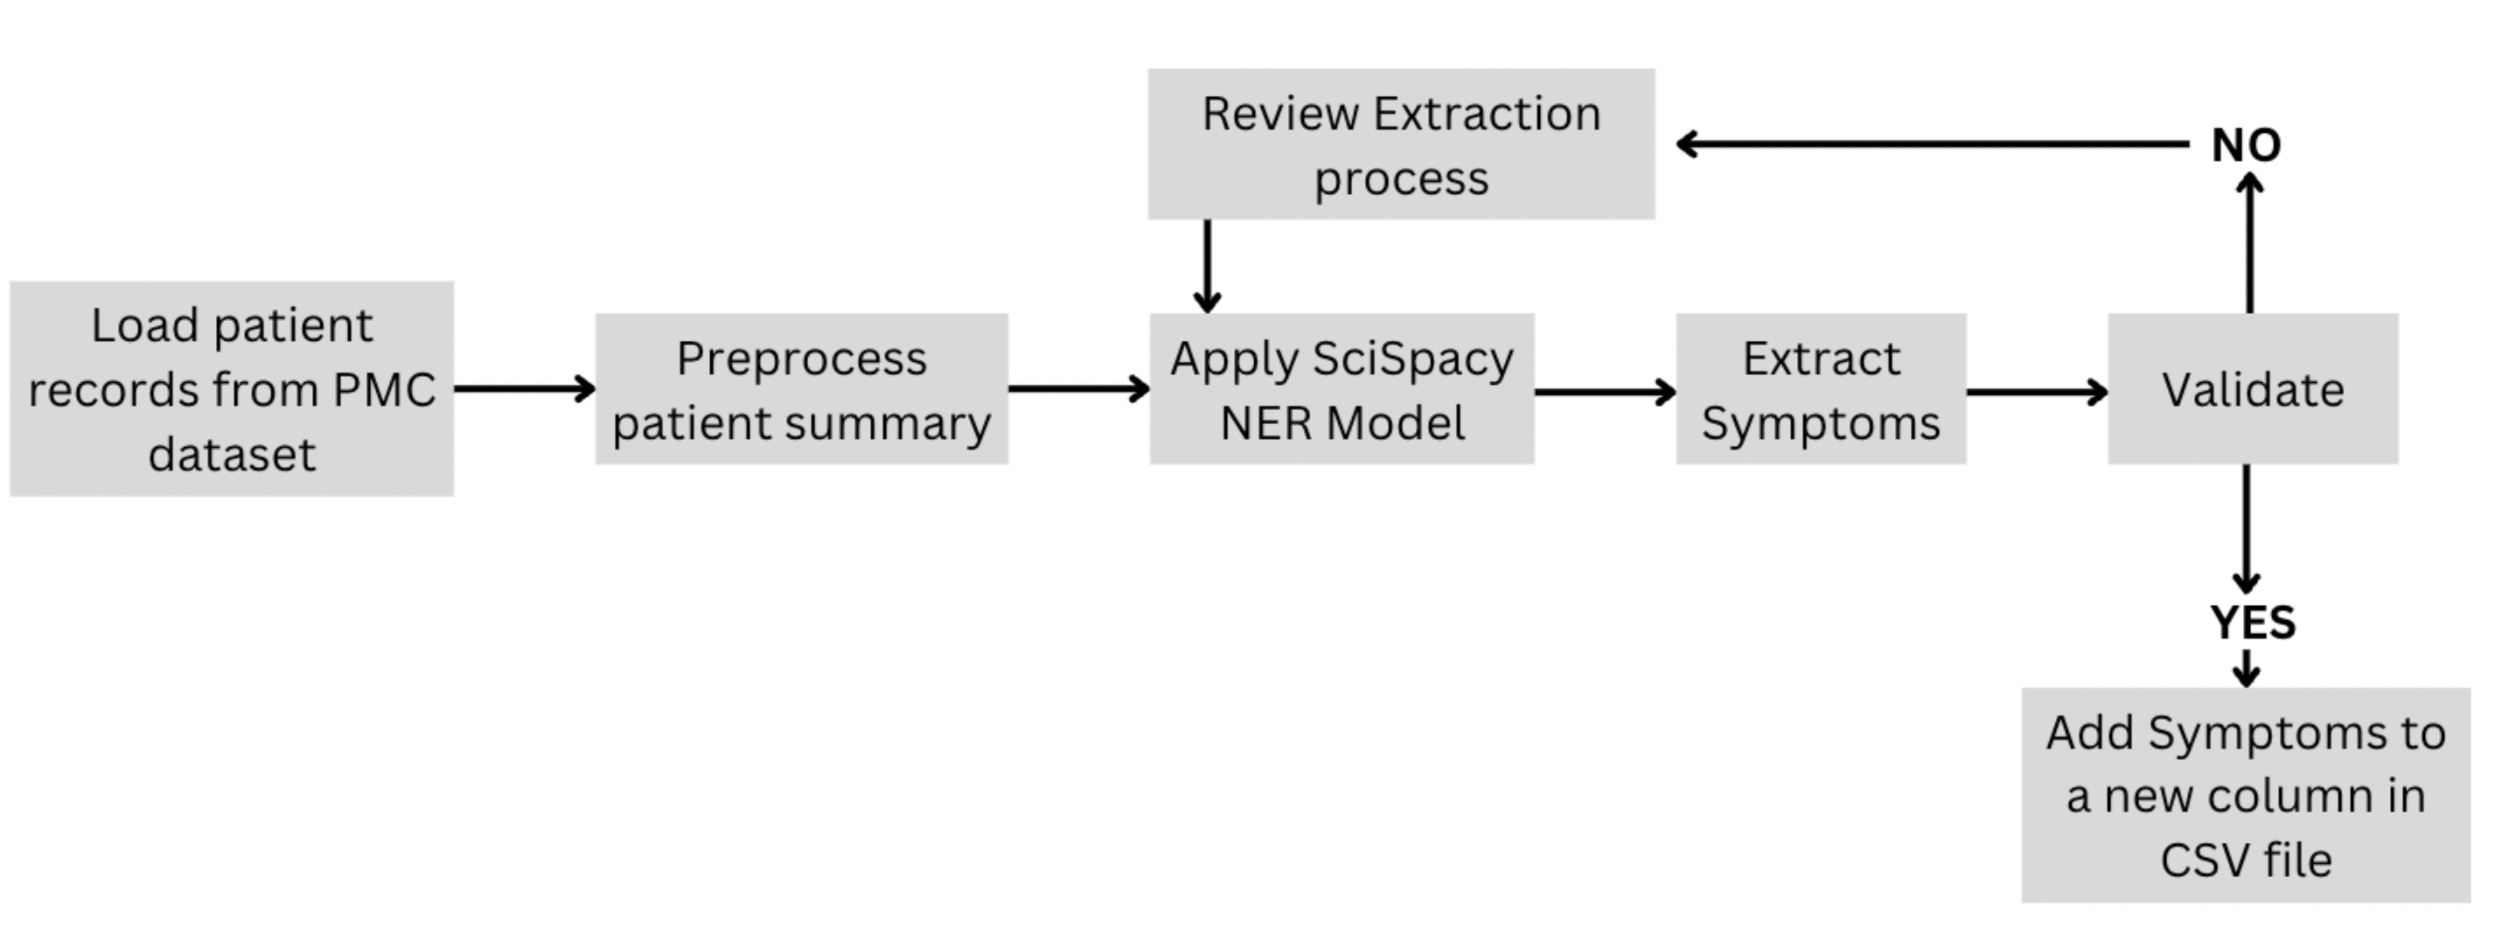
\includegraphics[width=0.8\textwidth]{fig/symptom_extraction.png}  
    \caption{Key steps in the symptom extraction process}
    \label{fig:symptom_extraction}
\end{figure*}

\subsection{Why Were the Models Chosen?}

SciSpaCy was selected due to its robust capabilities in biomedical text processing. Unlike generic NLP libraries, SciSpaCy is specifically designed to handle complex medical terminology, making it well-suited for symptom extraction. Key reasons for its preference include:

\begin{itemize}
    \item \textbf{Pre-Trained Medical Models}: SciSpaCy includes models trained on large-scale biomedical datasets, allowing for high-accuracy symptom recognition.
    \item \textbf{Integration with Medical Knowledge Bases}: It supports linking extracted terms to medical ontologies such as UMLS, enhancing reliability.
    \item \textbf{Scalability}: SciSpaCy is optimized for handling large datasets, making it ideal for processing extensive patient records.
    \item \textbf{Customization and Flexibility}: The framework allows for fine-tuning models and adding domain-specific rules, making it adaptable to various medical applications.
\end{itemize}

\subsection{Exceptional Cases}
Consider the following example medical string from our dataset:

\begin{quote}
\textit{“Early Physical Therapist Interventions for Patients With COVID-19 in the Acute Care Hospital: A Case Report Series." This 60-year-old male was hospitalized due to moderate ARDS from COVID-19 with symptoms of fever, dry cough, and dyspnea. We encountered several difficulties during physical therapy on the acute ward. First, any change of position or deep breathing triggered coughing attacks that induced oxygen desaturation and dyspnea. To avoid rapid deterioration and respiratory failure, we instructed and performed position changes very slowly and step-by-step. In this way, a position change to the 135° prone position took around 30 minutes. This approach was well tolerated and increased oxygen saturation. For example, on day 5 with 6 L/min of oxygen, his saturation improved from 93\% to 97\%. Second, we had to adapt the breathing exercises to avoid prolonged coughing and oxygen desaturation. Accordingly, we instructed the patient to stop every deep breath before the need to cough and to hold inspiration for better air distribution. In this manner, the patient performed the breathing exercises well and managed to increase his oxygen saturation. Third, the patient had difficulty maintaining sufficient oxygen saturation during physical activity. However, with close monitoring and frequent breaks, he managed to perform strength and walking exercises at a low level without any significant deoxygenation. Exercise progression was low on days 1 to 5 but then increased daily until hospital discharge to a rehabilitation clinic on day 10.”}
\end{quote}

The model correctly extracts symptoms such as \textbf{'dry cough,' 'dyspnea,' 'cough,' 'coughing,'} and \textbf{'COVID-19'}. However, it also incorrectly identifies non-symptoms such as \textbf{'acute ward,' 'air distribution,' 'physical therapy,'} and \textbf{'position'}. 

To improve symptom extraction, refining the model's training data and incorporating domain-specific filtering techniques can help reduce false positives. Additionally, handling ambiguous terms and context-dependent cases—such as distinguishing 'position' in a medical posture versus a symptom-related description—can further enhance accuracy.

\subsection{Encoder}
The goal of our encoder is to take the symptoms of the patients as input and to predict the relevant articles for these symptoms.\\
As our encoder, we used a RoBERTa model~\cite{liu2019robertarobustlyoptimizedbert}, which is an optimized BERT model~\cite{devlin2018bert}, which on the other hand is a transformer encoder stack~\cite{vaswani2017attention}. The input of our model are tokens of the symptoms that are calculated using the RoBERTA tokenizer. Since the task was to classify the symptoms, we used RobertaForSequenceClassification which is a module in PyTorch.\footnote{\url{https://huggingface.co/docs/transformers/model_doc/roberta}} It contains a normal RoBERTa model with a linear layer on top, so that the output is already logits. These logits are then sent through a sigmoid activation function to get a probability distribution over all possible papers. We then applied Top-K sampling to extract the k most probable papers, for the given symptoms.

\subsection{Training}
For training the encoder model, we split the dataset into training and test sets with a ratio of 80/20. The batch sizes depended on the size of the training data. Over time we had training data with different input and output sizes depending on how many papers we used and if we used only symptoms or whole patient descriptions as the input. The patient descriptions often exceeded the input length maximum from the RoBERTa-tokenizer of 512 tokens while the length of the extracted symptoms stayed under 50 tokens most of the time. Since we trained our model on a NVIDIA GeForce RTX 2080 Super with 8GB of GDDR6 VRAM our computational power was limited and by exhausting the computational limits, the batches varied in sizes between 16 and 256, depending on the mentioned training data. The size also effected the training duration and was between 19 seconds and 150 minutes per epoch, which resulted in complete training durations of about 16 minutes for 50 epochs and theoretically over 5 days, which we were not able to do, since we could not let our model train for over 5 days on our private hardware.\\
We trained the model to minimize the binary cross entropy loss function. PyTorch has a variation, that already has a sigmoid activation function implemented, that is called BCEWithLogitsLoss. Therefore, we could feed the encoder output directly into the loss function. It is also numerically more stable to combine both steps into one layer, because it takes advantage of the log-sum-exp trick for numerical stability.\footnote{\url{https://pytorch.org/docs/stable/generated/torch.nn.BCEWithLogitsLoss.html}} Since the total number of papers were significantly higher than the number of papers per patient we had to apply a custom positive weight to each paper in the loss function according to the formula:
\begin{align*}
    pos\_weight = \frac{n_t - n_a}{n_a}
\end{align*}
%posweight=(n_t-n_a  )/n_a 
were $n_t$ denotes the total number of papers and $n_a$ denotes the average number of papers per patient.
As an optimizer we used the Adam optimizer~\cite{diederik2014adam} with a learning rate of 0.0001. As seen in Figure~\ref{fig:loss} our model immediately began to overfit. This is due to the high number of different papers. Since there are nearly 3 times more papers than patients, there are lot of papers in the test dataset that are not in the train dataset. Therefore, the model is not able to predict these papers and the test loss gets worse over time.

\begin{figure}[hbt!]
    \centering
    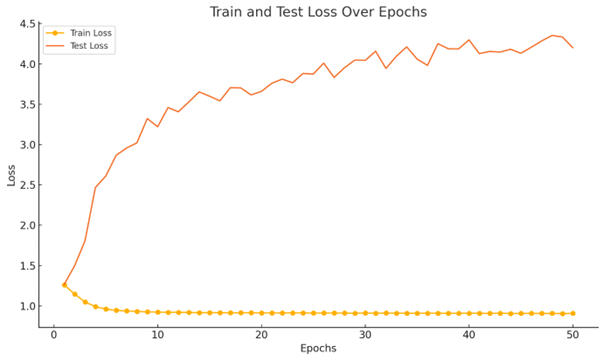
\includegraphics[width=0.5\textwidth]{Fig/loss.png}
    \caption{Train- and test-loss during training of the RoBERTa model}
    \label{fig:loss}
\end{figure}\noindent 

\subsection{Decoder}
To retrieve the corresponding full-text papers from the output of the encoder, which is a list of indices, the previously created mapping of paper IDs to indices is reused. Using this mapping, the list of paper IDs is obtained, and their respective full-text information is extracted from the full-text CSV by matching the paper IDs.
Since the full-text papers can span multiple pages, making their content accessible and understandable in a short time frame requires summarization. This allows users to quickly grasp the key insights of each paper without having to read them in full.
A variety of decoder language models (LLMs) were considered for this task, including Mistral, LLaMA 2, and LLaMA 3.3. However, due to hardware constraints, LLaMA 3.2 1B Instruct was ultimately chosen. Before passing the full-text papers to the LLaMA model for summarization, additional considerations were necessary to manage hardware limitations effectively.
To optimize memory usage, the RoBERTa model was re-initialized with each patient summary input and deleted before using the LLaMA model. This approach resulted in a negligible trade-off between initialization time and memory usage. Furthermore, instead of processing each full-text paper as a whole, the papers were split into halves to accommodate the GPU's memory limitations.
Each section of a paper was appended to a structured prompt containing summarization instructions. Once all papers and their respective sections were processed, the prompt was removed from each summary. The summarized sections of each paper were then concatenated to reconstruct a single coherent summary per paper. Finally, all individual paper summaries were combined into a single output string before being returned to the user interface.

\subsection{Evaluation methods}
For measuring medical text summarization quality, a set of proven metrics is used. The metrics assess different aspects of the generated summaries, including lexical similarity, phrase accuracy, fluency, semantic relevance, and synonym detection. The particular evaluation methods and how they are used in medical summarization are described below.
\begin{enumerate}

\item \textbf{BLEU} (Bilingual Evaluation Understudy)
Application: BLEU measures similarity between generated summary and reference text in terms of n-gram overlaps. It employs precision-scaled scoring, wherein n-grams in the generated text are matched with n-grams in the reference text, and a brevity penalty is used to avoid very short summaries.
\\
Procedure:
Tokenize generated summary and reference text.
Get unigrams, bigrams, trigrams, and higher-order n-grams.
Calculate overlapping n-gram precision.
Apply a brevity penalty if the summary is less than the reference.
\\
Applicability to Medical Summarization: BLEU can preserve key medical terms and phrases unaltered in the summary. However, since it computes exact word overlaps, at times it may also lose the overall meaning, which is extremely crucial in medical environments where synonym use is widespread.
\\
    \item \textbf{ROUGE-1} (Recall-Oriented Understudy for Gisting Evaluation - Unigram Overlap)
Application: ROUGE-1 estimates the frequency of unique keywords by calculating the recall of intersecting unigrams between the generated summary and the reference text.
\\
Procedure:
Both texts are tokenized.
Compute the number of matching unigrams between the reference and generated summaries.
Compute recall by dividing the number of overlapping unigrams by the number of reference summary unigrams.
\\
Relevance to Medical Summarization: The measure ensures the most important medical keywords, i.e., the diagnoses, treatments, and symptoms, are reflected in the summary. It confirms no important words are omitted, as is desired in medical reporting.
\\
    \item \textbf{ROUGE-2} (Bigram Overlap)
Use: ROUGE-2 measures phrase-level accuracy using bigram (two-word) overlap between system output and reference summaries.
\\
Procedure:
Tokenize both summaries.
Find bigrams from both summaries.
Compute recall as the number of exact bigrams over the total number of bigrams in the reference summary.
\\
Medical Summarization Relevance: By considering matches at the phrase level, this metric helps us assess the contextually correct usage of medical phrases, such that medically significant expressions like "chronic kidney disease" are correctly captured in the summary.
\\
    \item \textbf{ROUGE-L} (Longest Common Subsequence)
Application: ROUGE-L measures the longest common subsequence of words between the generated abstract and reference text with original word order. This is employed to measure fluency and sentence construction.
\\
Procedure:
Identify the longest common subsequence (LCS) of the two texts.
Compute recall and F1-score based on the LCS length.
\\
Relevance to Medical Summarization: This metric ensures that the generated summary is uniform and of the same sentence structure as complex medical sentences, which is crucial for clinical report and note readability and logical flow.
\\
    \item \textbf{METEOR} (Metric for Evaluation of Translation with Explicit ORdering)
Application: METEOR is an extension of BLEU with incorporation of synonyms, stemming, and word order along with explicit n-gram overlap. It is particularly useful in medical texts where different words share the same meaning.
\\
Procedure:
Tokenize text and apply stemming to normalize word forms.
Search for exact, stemmed, and synonym matches.
Compute a harmonic mean of precision and recall with additional penalties on incorrect word order.
\\
Relevance to Medical Summarization: METEOR is helpful in detecting the semantic similarity of medical terminology (e.g., "hypertension" and "high blood pressure"). This helps to ensure that variation in medical vocabulary is taken into account, leading to improved estimation of summary quality.
\\
    \item \textbf{BERTScore}
Application: BERTScore employs transformer-based embeddings to measure the semantic similarity between the reference and generated summaries, rather than word or phrase matching.
\\
Procedure:
Embed both summaries within the context of a pre-trained BERT model.
Compute cosine similarity between token embeddings.
Average token-level scores to produce a global similarity score.
\\
Relevance to Medical Summarization: BERTScore ensures that the complex medical information present in the summary maintains its original meaning. Since medical text often involves subtle details, this metric avoids the global message being altered even when different wording is used.
Using these evaluation criteria, this work ensures that the generated medical summaries are very lexically accurate, semantically true, fluent, and recall-high of critical medical information. Each criterion serves a specific purpose in assessing medical summarization quality:
BLEU and ROUGE assess key term recall.
ROUGE-2 and ROUGE-L assess phrase-level precision and fluency.
METEOR accounts for variations in medical jargon.
BERTScore ensures semantic preservation of intricate medical information.
This integrated assessment system helps ensure that medical summaries are informative, accurate, and beneficial for clinical and research purposes.
\end{enumerate}

\section{Results}
The system performs modestly, but it is not very accurate as most scores are below 0.7, indicating a room for improvement.
 BLEU (0.503) - Moderately shows word-for-word accuracy but is relatively low, indicating that the system is poor at exact matches.
ROUGE-1 (0.639) \& ROUGE-2 (0.574) - Indicate that the system is to a certain extent capturing significant words and phrases but without good recall.
ROUGE-L (0.582) - Means that the text generated is structurally coherent to a certain degree but is not accurate to a great extent.
METEOR (0.671) - Better than BLEU and ROUGE since it takes synonyms into consideration, but anything less than 0.7 indicates that semantic accuracy is not high.
BERTScore (0.768) - The highest of all, suggesting that the system is more capable of capturing semantic meaning than lexical matching, but even this score suggests that there is plenty of room for improvement.
Comparisons \& Conclusion
Overall Performance: The system does not do very well as most scores are below 0.7, suggesting that it is not very accurate in lexical and semantic matching.
Weaknesses: BLEU and ROUGE scores are low, indicating that the generated output does not adhere to reference text closely, either in exact words or in structure.
Strengths: The system is relatively better in semantic understanding (BERTScore), but even this is not high enough to be consistently strong.
Conclusion: The system's performance is at best fair but not accurate enough. It performs badly on exact matches, recall, and structural coherence, and word choice and semantic alignment must be improved to achieve higher scores.

\section{Discussion}
This work presented a two-stage approach (retrieval and summarization) for clinical decision support by integrating symptom extraction, document retrieval, and text summarization. Our results indicate that while the model demonstrates a reasonable ability to capture the overall semantic content—as reflected by a comparatively higher BERTScore—the lexical and structural accuracy, as measured by BLEU and ROUGE metrics, leaves considerable room for improvement.\\
One of the key observations is the discrepancy between semantic similarity and exact textual matching. Although the model appears to understand and retain the underlying medical context, it struggles to replicate the precise wording and structure of the reference texts. This divergence is critical in clinical settings, where even subtle changes in phrasing can lead to misinterpretation of important information. Future work should explore strategies to better balance semantic fidelity with lexical accuracy, perhaps by refining the loss function or employing more sophisticated fine-tuning techniques.\\
In our current approach, we used a RoBERTa-based classification model for retrieving relevant papers based on patient symptoms. However, an alternative strategy worth considering is the Retrieval-Augmented Generation (RAG) framework. RAG integrates retrieval directly into the generation process, potentially allowing for a more seamless integration between relevant document context and the generated summaries. This approach could mitigate some of the limitations observed with the RoBERTa classifier, such as overfitting due to the high number of paper labels relative to patient cases. Experimenting with RAG may improve both the accuracy of the retrieval step and the coherence of the final summaries.\\
The overfitting observed during training, likely caused by the high number of paper labels relative to patient cases, further underscores the challenges inherent in this domain. Limited hardware resources imposed additional constraints on batch sizes and training durations, potentially hindering the model’s ability to generalize to unseen data. Scaling up the training process with more robust computational resources or implementing more effective regularization techniques could help mitigate these issues. Additionally, employing a different dataset—ideally one with a more balanced label distribution or higher quality annotations—could further improve training outcomes and enhance the model’s generalizability.\\
The symptom extraction module, which relies on SciSpaCy, performed adequately in capturing medically relevant terms but also produced false positives—misidentifying terms that are contextually ambiguous. While the use of domain-specific pre-trained models like SciSpaCy is a step in the right direction, incorporating additional filtering mechanisms or ensemble approaches may be necessary to enhance accuracy and reduce noise in the extracted data.\\
Despite these challenges, the project's work shows promise. The model’s ability to generate semantically coherent summaries suggests that, with further refinements and possibly the adoption of a RAG-based retrieval strategy, it could become a valuable tool for clinicians overwhelmed by the growing volume of medical literature. Future iterations might benefit from experimenting with more advanced LLMs and larger, more diverse datasets to improve both retrieval and summarization performance.\\
Finally, while standard metrics like BLEU, ROUGE, and METEOR provide useful quantitative insights, they may not fully capture the clinical relevance of the summaries. Incorporating qualitative evaluations from medical professionals and conducting user studies will be essential to validate the system’s practical utility and ensure that the generated summaries meet the high standards required in clinical decision-making.\\
In summary, our work lays the groundwork for leveraging fine-tuned language models in clinical decision support but also highlights several critical areas—such as overfitting, hardware limitations, and symptom extraction accuracy—that need to be addressed. The insights gained from this work will guide future project toward developing more robust and clinically applicable AI tools.

\section{Contributions}

Authors names ordered by surname\\
\\
\textbf{Data Preparation}\\
Neil Hinrichs, Willi Löther, Dominik Martens, Tejaswi Venkatesh
\\
\textbf{Data Retrieval}\\
Willi Löther, Dominik Martens
\\
\textbf{Decoder}\\
Neil Hinrichs, Willi Löther, Dominik Martens
\\
\textbf{Document Text}\\
Neil Hinrichs, Willi Löther, Dominik Martens
\\
\textbf{Encoder}\\
Neil Hinrichs
\\
\textbf{Evaluation}\\
Tejaswi Venkatesh
\\
\textbf{LaTeX Document Preparation}\\
Neil Hinrichs, Willi Löther, Tejaswi Venkatesh
\\
\textbf{Presentation}\\
Neil Hinrichs, Willi Löther, Dominik Martens, Tejaswi Venkatesh
\\
\textbf{Symptom Extraction}\\
Dominik Martens
\\
\textbf{Training}\\
Neil Hinrichs
\\
\textbf{Web UI}\\



%\bibliographystyle{plain}
%\bibliography{reference}

%\begin{thebibliography}{10}

%\bibitem{bahdanau2014neural}
%Dzmitry Bahdanau, Kyunghyun Cho, and Yoshua Bengio.
%\newblock Neural machine translation by jointly learning to align and
%  translate.
%\newblock {\em arXiv preprint arXiv:1409.0473}, 2014.

\bibliographystyle{plain}
\bibliography{reference}
%\printbibliography[heading=bibintoc,title={References}]

%\end{thebibliography}

\end{document}